%%%% Proceedings format for most of ACM conferences (with the exceptions listed below) and all ICPS volumes.
% * <vipinkmenon@gmail.com> 2017-11-21T15:54:24.761Z:
%
% ^.
\documentclass[conference,10pt,a4paper]{IEEEtran}
\IEEEoverridecommandlockouts
%%%% As of March 2017, [siggraph] is no longer used. Please use sigconf (above) for SIGGRAPH conferences.

%%%% Proceedings format for SIGPLAN conferences 
% \documentclass[sigplan, anonymous, review]{acmart}

%%%% Proceedings format for SIGCHI conferences
% \documentclass[sigchi, review]{acmart}

%%%% To use the SIGCHI extended abstract template, please visit
% https://www.overleaf.com/read/zzzfqvkmrfzn


\usepackage{booktabs} % For formal tables
\usepackage{graphicx}
\usepackage{amsmath,amssymb,amsfonts}
\usepackage{algorithmic}
\usepackage{subfigure}

% Copyright
%\setcopyright{none}
%\setcopyright{acmcopyright}
%\setcopyright{acmlicensed}
%\setcopyright{rightsretained}
%\setcopyright{usgov}
%\setcopyright{usgovmixed}
%\setcopyright{cagov}
%\setcopyright{cagovmixed}

\begin{document}

\title{Revisiting Binary trees for efficient FPGA-based NoC implementation}

%\author{\IEEEauthorblockN{Kizheppatt~Vipin}
% \IEEEauthorblockA{Department of Electrical and Computer Engineering\\
%  Nazarbayev University, Astana, Kazakhstan \\
%  email:vipin.kizheppatt@nu.edu.kz
% }
%}
\maketitle

\begin{abstract}
Binary tree topology generally fails to attract network on chip (NoC) implementations due to its low bisection bandwidth.
Fat trees are used to alleviate this issue by using increasingly thicker links to connect switches towards the root node.
This scheme is very efficient in interconnected networks such as in computer networks, which uses generic switches for interconnecting compute nodes.
In an NoC context especially for field programmable gate arrays (FPGAs), fat trees require more complex switches as we move higher in the hierarchy which restricts the maximum clock frequency at which the network can operate.
This can offset the higher bandwidth achieved through using fatter links.
In this paper we discuss the implementation of a binary tree based NoC implementation, which achieves better bandwidth by varying the clock frequency between the switches as we move higher in the hierarchy.
This scheme enables using simpler switch architecture enabling higher maximum frequency of operation.
The effect on bandwidth and resource requirement of this architecture is compared with fat tree implementation for different number of nodes and different network traffic patterns.
\end{abstract}

\begin{IEEEkeywords}
network on chip, topology, binary tree, FPGA
\end{IEEEkeywords}


\section{Introduction}
Network on Chip (NoC) architectures enable high performance, scalable and power efficient multi-core systems for modern compute and communication intensive applications.
Researchers have proposed different NoC topologies such as mesh, ring, torus, binary trees, star etc., each having varying degrees of quality of service, bandwidth and latency~\cite{Dally2003}.
Despite their simple architecture and routing algorithms, binary trees are generally not attractive for NoC implementations.
It is mainly because of its lower bisection bandwidth.
Fat trees are proposed as a remedy to improve the bandwidth by adding more number of links when moving towards the root node.
This solution works well in traditional interconnect networks such as computer networks~\cite{Shainer2011}.
In a NoC environment, their advantage is limited since more complex switches have to be used in higher hierarchy.
This limits the overall clock performance thus bringing down the system performance. 

Theoretically instead of increasing the link width between tree levels, increasing the clock frequency between them should provide the same benefit.
In traditional networks this may not be possible since the network interfaces operate on predefined standards which restricts the frequency of operation.
Modern FPGAs support asynchronous FIFOs, which makes the implementation of asynchronous switches easier.
These switches have architecture simpler than fat tree switches and supports better clock frequencies.
But they are more resource intensive compared to traditional binary trees.


\begin{figure}[t]
\centering
   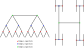
\includegraphics[width=0.8\columnwidth]{Figures/HNoC.pdf}
   \caption{(a)A binary tree topology utilizing switches operating at different clock frequencies (b) The tree as an H-tree for better floorplanning on the FPGA}
   \label{fig:btree}
   \vspace{-5 mm}
\end{figure}

Although asynchronous NoCs are proposed before for integrated circuits, a quantitative analysis is missing in the literature especially for FPGA implementations.
In this paper we present a quantitative analysis of different tree topologies namely the binary tree, binary fat tree and asynchronous binary tree when targeting FPGA based NoC implementation. 
The main contributions of this work are
\begin{itemize}
\item detailed design of an open-source globally asynchronous-locally synchronous (GALS) binary tree based NoC implementation targeting Xilinx FPGAs
\item performance evaluation of the proposed infrastructure with traditional binary trees and the state-of-the-art open source binary fat tree (CONNECT) and mesh topologies
\item analysis of trade-off points for the different implementations when targeting FPGAs
\end{itemize}
The remainder of this paper is organized as, Section~\ref{sec:background} discusses the relevant background, Section~\ref{sec:arch} discusses the architecture of the proposed NoC, Section~\ref{sec:result} discussed the performance metrics and ~\ref{sec:conclusion} concludes the paper and gives the future research directions.
\section{Background}
\label{sec:background}
Network on chip is an interconnect approach that helps different IPs and subsystems in a chip to communicate with each other in an efficient and scalable manner. 
In this approach each processing element (PE) is connected to a switch and multiple switches are interconnected to form a network.
A PE could be a processor core, a DSP core or an IP block.
The network infrastructure helps in routing data from one PE to another in the form of data packets. 
Based on how the switches are interconnected, there are different NoC topologies such as mesh, torus, tree, ring, star, BFT etc.
In a mesh topology every switch, except the ones on the edges, is connected to 4 other neighbouring switches.
A torus topology is similar to mesh but cyclic in nature.
In a binary tree, switches are arranged in a hierarchy.
Each switch has a parent node and two child nodes.
Unlike mesh and torus where each switch has a corresponding PE, in a tree topology only the switches at the bottom most level are connected to PEs.

An important network performance parameter is the bisection bandwidth.
It is defined as the minimum bandwidth between two equal partitions of the network.
For a mesh topology, it is $\sqrt{n}*B$, where n is the number of switches in the network and B is the bandwidth of a single link between switches.
For torus, it is twice that of mesh but for a binary tree, it is only B.
To address this issue, instead of using a single link between switches more links can be used between them as we go higher in the tree hierarchy.
Such topology is called a fat tree~\cite{Leiserson1985}. 
Although this will improve the bisection bandwidth, the switches in the upper hierarchy becomes more and more complex.
We analyze whether using asynchronous switches with same link width can provide similar performance of fat trees while keeping relatively simpler switches.
\section{Architecture}
\label{sec:arch}

AsyncBTree tries to achieve better performance compared to a conventional binary trees and fat trees in terms of resource utilization and throughput by applying FPGA and topology specific optimizations and using asynchronous links between different tree levels.
Fig.~\ref{fig:btree} shows the architecture of AyncBTree utilizing different kind of optimized switches at different levels.
The detailed architecture of the switches are discussed in Section~\ref{sec:switch}.
The binary tree is placed and routed in the FPGA as an H-tree for efficient resource utlization and better floorplanning.
Such placement also supports partial reconfiguration of a portion of the NoC in effieicnet manner.
As the first optimization, the root node of the tree is removed and the switches at level-1 are directly connected.
Since the connectivity of the root node is only 2, in practical systems they act as a transparent switch.
They could be useful where packets are injected to the NoC through the root node by making its connectivity as 3.
In FPGAs external interfaces such as PCI express and Ethernet are used for injecting packets.
The hardmacros corresponding to these cores are situated along the periphery of the chips.
Thus it will provide better clock performance when the packets are injected from one the leaf nodes which incorporates one of these hard macros.
Removing the root node helps in reducing the resource utilization.

\begin{figure}[t]
\centering
   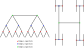
\includegraphics[width=\columnwidth]{Figures/HNoC.pdf}
   \caption{(a)A binary tree topology utilizing switches operating at different clock frequencies (b) The tree as an H-tree for better floorplanning on the FPGA}
   \label{fig:btree}
\end{figure}

\begin{figure}[t]
\centering
   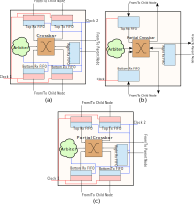
\includegraphics[width=\columnwidth]{Figures/switch1_2.pdf}
   \caption{Architecture of the different switches used in the AsyncBTree. (a) Type-1 switch used with the leaf nodes (PEs), with complete cross bar switch and asynchrnous 
   FIFOs with receive and transmit interfaces (b) Type-2 switch used in intermediate nodes with partial crossbar switch and synchronous FIFOs (c) Type-3 switches used in intermediate
   switches with partial cross bar and asynchrnous FIFOs with receive and transmit interfaces.}
   \label{fig:switchArch}
\end{figure}

\subsection{Switches}
\label{sec:switch}
AsyncBTree uses three different kinds of switches for packet routing.
The architecture of the proposed type-1 switch is as shown in Fig.~\ref{fig:switchArch}(a).
Type-1 switches are used only in the leaf nodes for directly interfacing with the PEs.
The switch has separate interface for receiving and transmitting packets from the two child nodes (PEs) and a single interface to the parent node.
Each receive and transmit interface to the PEs are connects to an asynchronous FIFOs.
The interface to the parent node contains a single synchronous FIFO for the receive interface and no transmit FIFO.
Thus each switch contains 5 FIFOs.

Asynchronous FIFOs can operate their read and write interfaces using independent clocks.
The depth of the FIFOs are kept very low (16) to reduce the resource utilization.
The asynchronous FIFOs receive data from the downstream ports on Clock 1 signal.
The received packets are routed to the appropriate output ports by an arbitrator through a cross-bar switch.
The read side of the receive FIFO, the write side of the transmit FIFO, the arbitrator and the cross bar works on Clock 2 signal, whose frequency will be much higher than that of Clock 1.
In order to mach the performance of a binary fat tree, Clock 2 frequency should be twice as that of Clock 1.

The arbitrator internally uses flit-level round-robin arbitration scheme to select the input port when more than one port requests for the same output port.
If a single port is requesting for a particular out, it is given the access until all the flits are sent out.

\subsection{Routing}
\label{sec:routing}
AyncBTree uses fixed routing based on the destination address of the packet header~\ref{fig:packet}.
The routing is flit level routing meaning each packet is expected to have the destination PE address in the packet header.
Larger packets are sent as multiple flits.
One major advantage of binary trees is the multiple packets sent from one PE to another will be always delivered in the sent order.
In other packet switched networks such as mesh or torus, the packets could be delivered in out of order depending on the routing algorithms.
In this case additional logic is required for packet reassembly and packet numbers also have to be inserted into the payload.

The routing table of each switch in AsyncBTree contains four entries corresponding to the smallest and largest PE addresses in its left sub-tree and right sub-tree.
If the destination address is with in the range of left sub-tree, it is routed left and if it is with in the range of right sub-tree the packet is sent right.
If the address is not within these ranges, the packet is routed towards the parent node.

\begin{figure}[t]
\centering
   
\includegraphics[width=\columnwidth]{Figures/pckt_structure.pdf}
   \caption{Packet structure}
   \label{fig:packet}
\end{figure}
\section{Results}
\label{sec:result}



\begin{figure*}[ht]
\centering     %%% not \center
\subfigure[Random]{\label{fig:a}\includegraphics[width=0.5\columnwidth]{Data/randomTput.pdf}}
\subfigure[Tornado]{\label{fig:b}\includegraphics[width=0.5\columnwidth]{Data/tornadoTput.pdf}}
\subfigure[Complement]{\label{fig:a}\includegraphics[width=0.5\columnwidth]{Data/complementTput.pdf}}
\subfigure[Reverse]{\label{fig:b}\includegraphics[width=0.5\columnwidth]{Data/reverseTput.pdf}}
\caption{Throughput of different Binary Noc architectures with varying size corresponding to different traffic patterns}
\end{figure*}

\begin{figure*}[ht]
\centering     %%% not \center
\subfigure[Figure A]{\label{fig:a}\includegraphics[width=0.5\columnwidth]{Data/randomLatency.pdf}}
\subfigure[Figure B]{\label{fig:b}\includegraphics[width=0.5\columnwidth]{Data/tornadoLatency.pdf}}
\subfigure[Figure A]{\label{fig:a}\includegraphics[width=0.5\columnwidth]{Data/complementLatency.pdf}}
\subfigure[Figure B]{\label{fig:b}\includegraphics[width=0.5\columnwidth]{Data/reverseLatency.pdf}}
\caption{Maximum latency of different Binary Noc architectures with varying size corresponding to different traffic patterns}
\end{figure*}

Table~\ref{table:systemResourceConsumption} compares the resource utilization and the maximum frequency of operation for HNoC and CONNECT for different number of PEs
\input Tables/SystemResource



\section{Conclusion}
\label{sec:conclusion}
In this paper we discussed the implementation of an asynchronous binary tree based NoC architecture targeting FPGA implementation.
Analysis shows that FPGA archtiecture specific optimization can provide high clock performance and low resource consumption for such implementation compared to traditional fat-tree based implementations.
It also shows the advantage of fixed size interface to PEs compared to variable size interface when targeting the NoC for partial reconfiguration.
Implementation of the proposed architecture is provided as an open source enabling other researchers to verify its functionality and to use in practical NoC-based applications~\cite{hnoc}.
In the future we will be anayzing the effect of GALS-based implementation of other network topologies when targeting FPGA implementations.



\bibliographystyle{IEEEtran}
\bibliography{nocs} 

\end{document}
